%!TEX encoding = UTF-8 Unicode  
\chapter{Tips:如何得到高质量的图片}

sda

\begin{figure}[htbp]
\begin{center}
	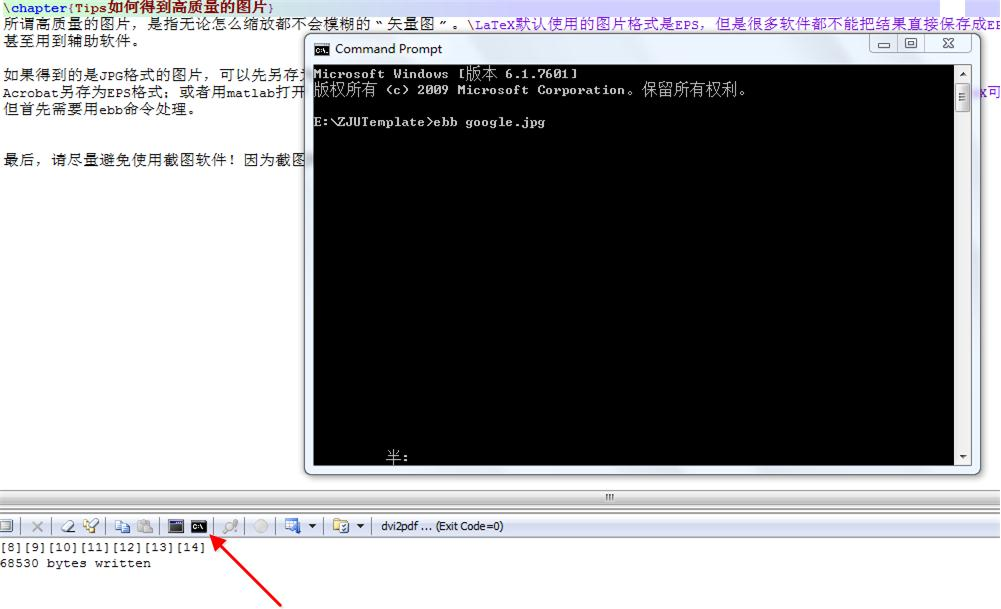
\includegraphics[width=0.8\linewidth]{command.jpg}
\end{center}
\caption{直接使用JPG图片}
\label{fig:google}
\end{figure}

如果得到的是pdf文件,可以先使用Adobe Acrobat的剪裁页面功能把图片周围的空白裁掉,再另存为EPS图片。

Adobe Illustrator软件可以将几乎任何格式图片另存为EPS图片。

如果要画流程图,或者对图片做修饰(如添加箭头、文本、图片的组合),可以使用软件Visio 2010.


最后,请尽量避免使用截图软件!因为截图得到的图片质量往往是很差的,经不起格式转换的折磨。




